\documentclass[border=0.5mm]{standalone}

\usepackage{tikz}
\usetikzlibrary{arrows.meta,positioning,fit,backgrounds,shapes}
\usepackage{xcolor}
\usepackage{amsmath}
\usepackage{amssymb}
\usetikzlibrary{pgfplots.groupplots}

\begin{document}

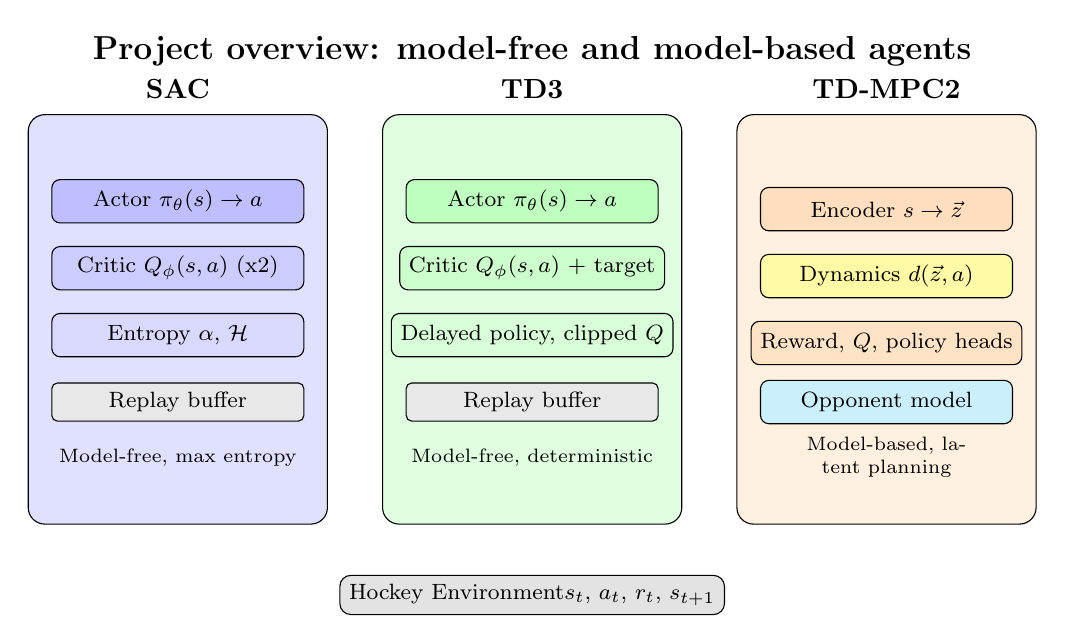
\begin{tikzpicture}[
  font=\sffamily,
  >=Stealth,
  algobox/.style={draw, rounded corners=6pt, minimum width=3.8cm, minimum height=5.2cm, align=center},
  component/.style={draw, rounded corners=3pt, minimum height=0.55cm, align=center, font=\footnotesize},
  sacbox/.style={fill=blue!12},
  td3box/.style={fill=green!12},
  tdmpcbox/.style={fill=orange!12},
  replay/.style={draw, rounded corners=2pt, fill=gray!18, font=\footnotesize},
  env/.style={draw, rounded corners=4pt, fill=gray!22, font=\footnotesize},
]

% Title
\node[font=\large\bfseries] (title) at (5.5, 3.4) {Project overview: model-free and model-based agents};

% Shared environment at bottom
\node[env, minimum width=4cm] (env_common) at (5.5, -3.5) {Hockey Environment\\$s_t$, $a_t$, $r_t$, $s_{t+1}$};

% ========== SAC (left) ==========
\def\xsac{1}
\node[algobox, sacbox] (sac_outer) at (\xsac, 0) {};
\node[font=\bfseries, above=2pt of sac_outer.north] {SAC};
\node[component, fill=blue!25, minimum width=3.2cm] (sac_actor) at (\xsac, 1.5) {Actor $\pi_\theta(s) \to a$};
\node[component, fill=blue!20, minimum width=3.2cm] (sac_critic1) at (\xsac, 0.65) {Critic $Q_\phi(s,a)$ (x2)};
\node[component, fill=blue!15, minimum width=3.2cm] (sac_entropy) at (\xsac, -0.2) {Entropy $\alpha$, $\mathcal{H}$};
\node[replay, minimum width=3.2cm] (sac_replay) at (\xsac, -1.05) {Replay buffer};
\node[font=\scriptsize, text width=3.4cm, align=center] at (\xsac, -1.75) {Model-free, max entropy};

% ========== TD3 (center) ==========
\node[algobox, td3box] (td3_outer) at (5.5, 0) {};
\node[font=\bfseries, above=2pt of td3_outer.north] {TD3};
\node[component, fill=green!25, minimum width=3.2cm] (td3_actor) at (5.5, 1.5) {Actor $\pi_\theta(s) \to a$};
\node[component, fill=green!20, minimum width=3.2cm] (td3_critic) at (5.5, 0.65) {Critic $Q_\phi(s,a)$ + target};
\node[component, fill=green!15, minimum width=3.2cm] (td3_delay) at (5.5, -0.2) {Delayed policy, clipped $Q$};
\node[replay, minimum width=3.2cm] (td3_replay) at (5.5, -1.05) {Replay buffer};
\node[font=\scriptsize, text width=3.4cm, align=center] at (5.5, -1.75) {Model-free, deterministic};

% ========== TD-MPC2 (right) ==========
\def\xtdmpc{10}
\node[algobox, tdmpcbox] (tdmpc_outer) at (\xtdmpc, 0) {};
\node[font=\bfseries, above=2pt of tdmpc_outer.north] {TD-MPC2};
\node[component, fill=orange!25, minimum width=3.2cm] (tdmpc_enc) at (\xtdmpc, 1.4) {Encoder $s \to \vec{z}$};
\node[component, fill=yellow!35, minimum width=3.2cm] (tdmpc_dyn) at (\xtdmpc, 0.55) {Dynamics $d(\vec{z},a)$};
\node[component, fill=orange!22, minimum width=3.2cm] (tdmpc_rqp) at (\xtdmpc, -0.3) {Reward, $Q$, policy heads};
\node[component, fill=cyan!20, minimum width=3.2cm] (tdmpc_opp) at (\xtdmpc, -1.05) {Opponent model};
\node[font=\scriptsize, text width=3.4cm, align=center] at (\xtdmpc, -1.75) {Model-based, latent planning};


\end{tikzpicture}
\end{document}
